\begin{flushright} {\tiny {\color{gray} python\_codes/fieldstone\_129/text.tex}} \end{flushright}

\lstinputlisting[language=bash,basicstyle=\small]{python_codes/fieldstone_129/keywords}

\begin{center}
\fbox{\textbf{\huge \color{teal} P}}
Codes at \url{https://github.com/cedrict/fieldstone/tree/master/python_codes/fieldstone_129}
\end{center}

\par\noindent\rule{\textwidth}{0.4pt}

%%%%%%%%%%%%%%%%%%%%%%%%%%%%%%%%%%%%%%%%%%%%%%%%%%%%%%%%%%%%%%%%%%%%%%%%%%%%%%%%%%%%%%%%%%%%%%

Following chapter 12 of Guy Simpson's book \cite{simp17} 
we have\footnote{I have slightly changed the notations.}

\[
\left(
\begin{array}{c}
\sigma_{xx}\\ 
\sigma_{yy}\\ 
\sigma_{xy} 
\end{array}
\right)
=
\left(
\begin{array}{ccc}
\frac{\delta t(4\mu \eta + 3K \eta+ 3K \mu\delta t)}{3(\mu \delta t + \eta)} &
\frac{\delta t(3K \eta+ 3K \mu\delta t - 2\mu \eta)}{3(\mu \delta t + \eta)} &
0 \\
\frac{\delta t(3K \eta+ 3K \mu\delta t  - 2\mu \eta)}{3(\mu \delta t + \eta)}&
\frac{\delta t(4\mu \eta + 3K \eta+ 3K \mu\delta t)}{3(\mu \delta t + \eta)} &
0  \\
0 & 0 & \frac{\mu \eta \delta t }{\mu \delta t + \eta}  \\
\end{array}
\right)
\cdot
\left(
\begin{array}{c}
\dot\varepsilon_{xx}\\ 
\dot\varepsilon_{yy}\\ 
{\color{teal}2}\dot\varepsilon_{xy} 
\end{array}
\right) 
+
\left(
\begin{array}{cccccc}
\frac13\frac{3\eta + \mu \delta t}{\mu\delta t+\eta} & 
\frac13\frac{\mu \delta t}{\mu\delta t+\eta} & 
0\\
\frac13\frac{\mu \delta t}{\mu\delta t+\eta} & 
\frac13\frac{3\eta + \mu \delta t}{\mu\delta t+\eta} & 
0\\
0 & 0 & \frac{ \eta}{\mu\delta t + \eta}  
\end{array}
\right)
\cdot
\left(
\begin{array}{c}
\sigma_{xx}^0\\ 
\sigma_{yy}^0\\ 
\sigma_{xy}^0 
\end{array}
\right) 
\]
We see that pressure is not a degree of freedom so the finite element
formulation and discretisation will not yield a saddle point problem, 
which is a good thing in terms of complexity and solving procedure.

In the end the following weak form is obtained:
\[
\int {\bm B}^T \cdot {\bm D} \cdot \tilde{\bm D} dV \cdot \vec{\cal V} 
= \int \vec{\bN} \rho \vec{g} dV -\int {\bm B}^T \cdot \tilde{\bm D}_s \cdot \vec{\sigma}_0 dV
\]

We need to keep track of the stress $\vec{\sigma}_0$ and 
we do so directly at the quadrature points.
The strain rate vector is recomputed at every time step but it is also 
directly stored on the quadrature points.

The current stress vector $\vec{\sigma}$ is also on the quadrature points and
is computed by means of the equation above.

In the end we declare the following arrays:
\begin{lstlisting}
nqperdim=3
nq=nel*nqperdim**ndim # total number of quadrature points
stress0_vector    = np.zeros((3,nq),dtype=np.float64) # stress vector memory
stress_vector     = np.zeros((3,nq),dtype=np.float64) # stress vector 
strainrate_vector = np.zeros((3,nq),dtype=np.float64) # strain rate vector
\end{lstlisting}

The code relies on quadratic elements ($Q_2$).
Each element is assigned a 'phase' (a material) and 
each material can have different values of $\mu, \eta, \nu, K, E$.

As is common when modelling elasto-viscous materials
we define an effective viscosity:
\[
\eta_{eff} 
= \frac{\eta \delta t}{\delta t + \eta/\mu} 
\]

When 
\[
\sigma_m 
= \frac{1}{3}(\sigma_{xx}+\sigma_{yy}+\sigma_{zz})
= \frac{1}{3}(\sigma_{xx}+\sigma_{yy}+\frac12(\sigma_{xx}+\sigma_{yy}))
= \frac{1}{2}(\sigma_{xx}+\sigma_{yy})
\]

The mesh deforms with the material flow (Lagrangian approach)
and this is simply implemented as follows 

\begin{lstlisting}
xV[:]+=u[:]*dt
yV[:]+=v[:]*dt
\end{lstlisting}



%------------------------------------------------------------------------------
\subsection*{Folding}

Boundary conditions are free slip on the left, right and bottom boundaries, while
a horizontal velocity of $\SI{5}{\mm\per\year}$ is prescribed on the right 
boundary\footnote{The vertical component of the velocity 
on the right wall is not clear, but looking at the figure we see that 
the thickening is the same on the left and right, so that the
vertical velocity on the right is unconstrained.}.
The formulation is such that there are only velocity degrees of freedom, no pressure.
Quadratic elements ($Q_2$) are used.

In the book, the time step is fixed to 
\[
\delta t = 0.01/edot = 0.01*Lx/u_{bc} = 0.01*4/5e-3 = 0.8year
\]

\begin{center}
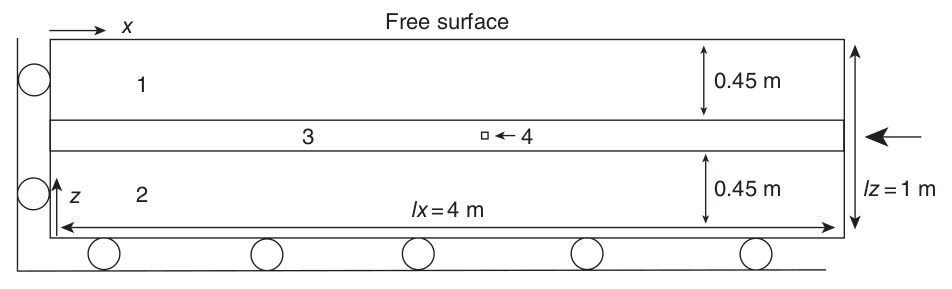
\includegraphics[width=13cm]{python_codes/fieldstone_129/images/simpson1}\\
{\captionfont  
Numbers indicate the lithological unit (termed the ``phase'' in the Matlab script). 
The folding experiment was
performed with a viscoelastic material where the central layer (i.e., phases 3 and 4) 
has a shear viscosity ($\eta=\SI{1e20}{\pascal\second}$) that
is 100 times greater than that of the surrounding matrix ($\SI{1e18}{\pascal\second}$). 
Other parameters are as follows: 
density = $\SI{2700}{\kg\per\cubic\meter}$ , 
gravity = $\SI{9.8}{\meter\per\square\second}$, 
Young's modulus = $\SI{1e11}{\pascal}$, 
Poisson’s ratio = 0.3 (all considered uniform throughout),
and a 40x40 elements.}
\end{center}


\begin{center}
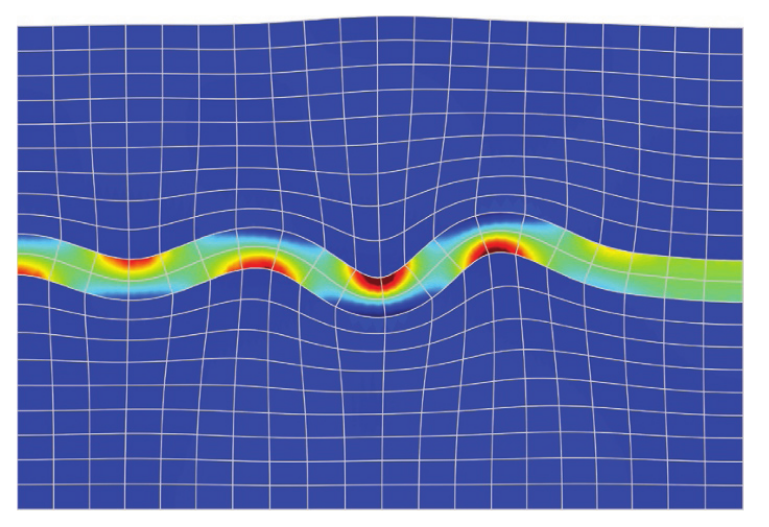
\includegraphics[width=10cm]{python_codes/fieldstone_129/images/simpson2}\\
{\captionfont 
Folding in a layered viscoelastic material after 40\% shortening. The central layer has a viscosity 100
higher than the surrounding matrix. The shaded colors represent mean stress, 
while the grid shows finite deformation (which is not the computational mesh).
Unfortunately no color legend.}
\end{center}

what about pre-stress, initial compaction?

Remark:
- p191, viscosity values in 1) are wrong ? different?


\begin{center}
\includegraphics[width=5.7cm]{python_codes/fieldstone_129/results/experiment1/result}
\end{center}

\begin{center}
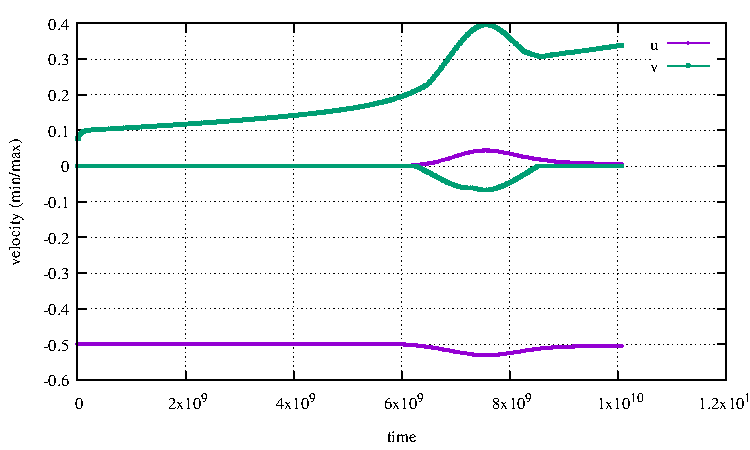
\includegraphics[width=5.7cm]{python_codes/fieldstone_129/results/experiment1/stats_velocity}
\includegraphics[width=5.7cm]{python_codes/fieldstone_129/results/experiment1/stats_strainrate}
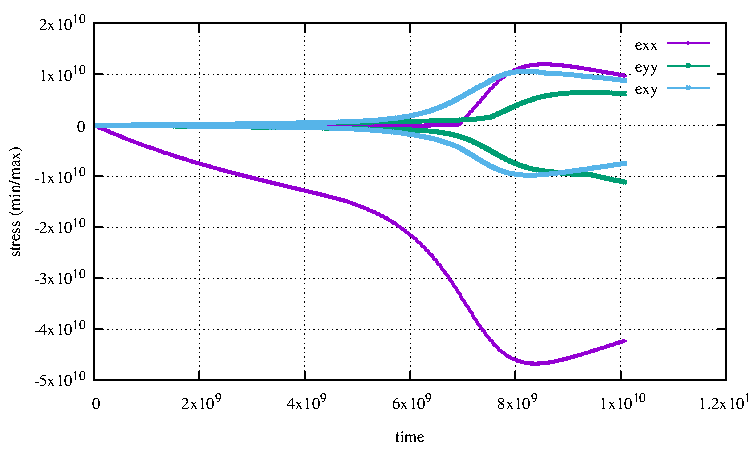
\includegraphics[width=5.7cm]{python_codes/fieldstone_129/results/experiment1/stats_stress}\\
{\captionfont a}
\end{center} 

%------------------------------------------------------------------------------
\subsection*{Numerical benchmark - pure/simple shear?}

The domain is $\SI{50}{\km}\times\SI{50}{\km}$. There is a single 
material in the domain characterised by $\eta=\SI{1e21}{\pascal\second}$,
$\mu=\SI{1e10}{\pascal}$. The time step is $\delta t=100~\si{\year}$.
Boundary conditions are free slip on all sides, with $u=+\SI{1}{\cm\per\year}$
on the right and $v=-\SI{1}{\cm\per\year}$ on the top.

The unstressed, {\it incompressible} viscoelastic Maxwell medium is subjected to a velocity field 
resulting in pure shear. 
The increase of the accumulated stress with time is given by an analytical solution:
\begin{equation}
{\bm \tau} 
= 2\eta\ {\dot{\bm \varepsilon}} \left ( 1-\exp\left(-\frac{\mu }{\eta} t \right) \right )
= 2\eta\ {\dot{\bm \varepsilon}} \left ( 1-\exp\left(-\frac{t}{t_M} \right) \right )
\end{equation}
where the Maxwell time is $t_M = \frac{\eta}{\mu} = \SI{1e11}{\second} \simeq 3171~\si{\year}$.

\begin{center}
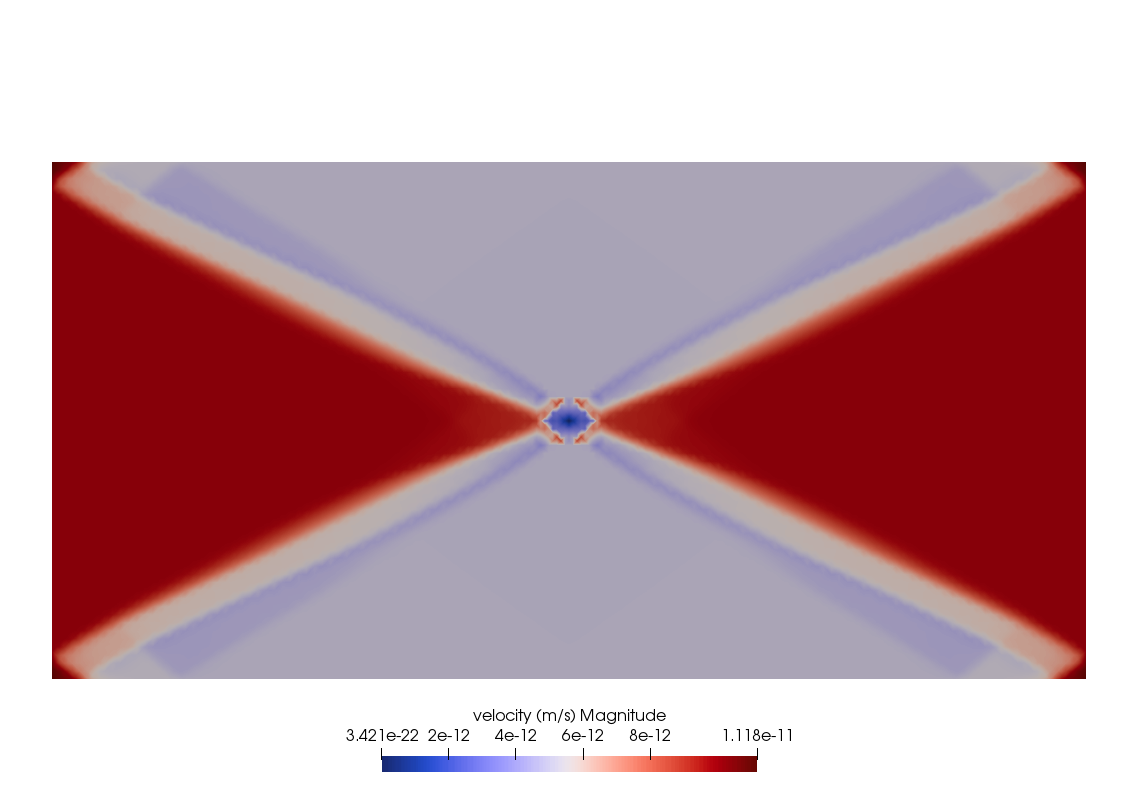
\includegraphics[width=5.7cm]{python_codes/fieldstone_129/results/experiment1/vel}\\
{\captionfont Velocity field.}
\end{center}

We have 
\[
\eta_{eff} 
= \frac{\eta \delta t}{\delta t + \eta/\mu} 
= \frac{10^{21} \cdot 3.154\times 10^{9}}{3.154\times 10^{9} + 10^{21}/10^{10}} 
\simeq 
\SI{3.0592e19}{\pascal\second} 
\]

The first time that the Stokes system is solved, there is no stored stress, i.e. the 
$\vec{\sigma}_0$ rhs is identically zero, so that the system is solved with a viscosity equal to
$\eta_{eff}$. 
We can easily compute the analytical solution, and we see that $\dot{\varepsilon}_{xy}=0$


\begin{center}
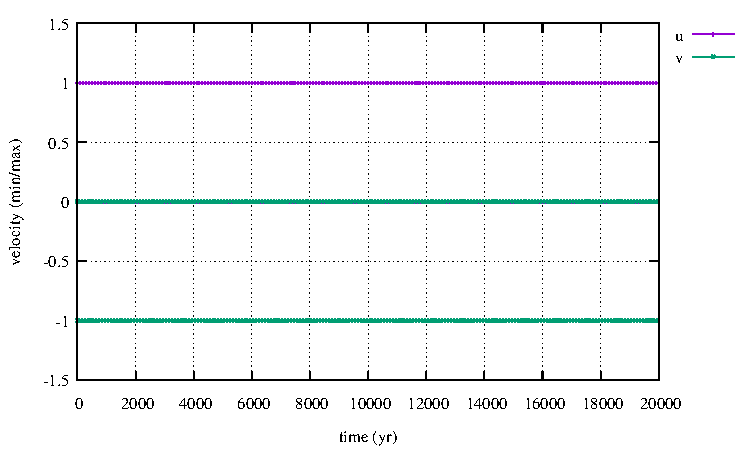
\includegraphics[width=5.7cm]{python_codes/fieldstone_129/results/experiment2/stats_velocity}
\includegraphics[width=5.7cm]{python_codes/fieldstone_129/results/experiment2/stats_strainrate}
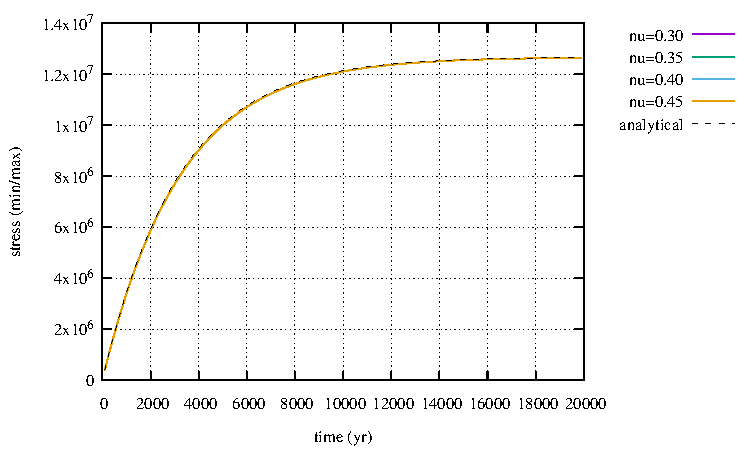
\includegraphics[width=5.7cm]{python_codes/fieldstone_129/results/experiment2/stats_stress}\\
{\captionfont Evolution of velocity, strain rate and stress statistics over 20~kyr.}
\end{center} 


TRY different POISSSON!


